\documentclass[12pt]{article}
\usepackage[left=1in, right=1.0in, top=1.0in,bottom = 1.0in]{geometry}
\usepackage{amsmath}
\usepackage{xcolor}
\usepackage{lmodern}
\usepackage{listings}
\usepackage{graphicx}
\usepackage{float}
\usepackage{mathtools}
\usepackage{pdfpages}

\lstset{language=[90]Fortran,
  basicstyle=\ttfamily,
  keywordstyle=\color{red},
  commentstyle=\color{blue},
  showstringspaces=false,
  morecomment=[l]{!\ }% Comment only with space after !
}


\begin{document}
	\begin{flushleft}
		Max Le \\
		ID: 901223283\\
		MTH 5050: Parallel Process\\
		Assignment 3: Matrix Vector Multiplication using OPENMP and MPI  
    \end{flushleft}


    \section{Problem Statement}

    The goals of this assignment are to use OPENMP and MPI to perform a series of matrix-vector multiplications. This is done in order to simulate the Google's Pagerank problem. We are going to start with a matrix S, which looks something like this: 

    \[
        S = \begin{pmatrix}
        0 & 0.5 & \dots & \dots & 0 \\
        0.5 & 0 & \dots & \dots & 0 \\
        \vdots & \vdots & \ddots & \dots & \vdots \\
        0 & 0 & \dots &  \ddots &\textbf{1.0} \\
        \textbf{0.5} & 0  & \dots & 0.5 & 0
        \end{pmatrix}
    \]
    \noindent
    In other words, this matrix S is a modified tri-diagonal matrix whose main diagonal contains 0, super and subdiagonal contain  0.5.  For the special points, the last entry of the superdiagonal is 1.0, as indicated as bold. The other special point is in the first column, the last entry is 0.5. This matrix S is used to set up matrix G, which is given by the following: 

    \begin{equation}
        G = (1-q)S + qB
    \end{equation}

    \noindent
    where q = damping factor = 0.15 and B is a constant matrix, the constant is the inverse of the PageNumber.  This "PageNumber" is an artificial representation of the size of the internet. In our problem, PageNumber = column/row size of matrix, which is 16 for the small problem and 1600 for the larger problem. In other words, B looks like this: 

    \[
        B = \begin{pmatrix}
          1/ncol & 1/ncol & \dots & 1/ncol \\
          1/ncol & 1/ncol & \dots & 1/ncol \\
          \vdots & \vdots & \ddots & \vdots \\
          1/ncol & 1/ncol & \dots & 1/ncol
        \end{pmatrix}
    \]

    \noindent
    We are going to multiply G by the vector x, which is a vector of constant $\dfrac{1}{PageNumber}$, similar to the matrix B. 


    \[
        X = \begin{pmatrix}
          1/ncol\\
          \dots \\
          \dots \\
          1/ncol
        \end{pmatrix}
    \]

    \noindent
    The resultant vector is called Y. We will then update X = Y, and perform the matrix multiplication again for 1000 times.
    
    \newpage
    \section{Approaches}
    The matix multiplication will be done in three different approaches. The first one is the dense approach, where we build and store G as a dense matrix; this will be done using OPENMP. The second approach is via CSR matrix; this will also be done in OPENMP. The last approach is in MPI and it involves building up the S matrix row by row. Brief details for each approach are discussed below

    \subsection{PART A: OPENMP DENSE}
    This is self-explanatory as we only need to build the entire G matrix. The OPENMP directives are added to the main matrix multiplication section. The first set of directives is added as a "PARALLEL DO PRIVATE" when we calculate the y vector, and the second set of directives is added to when we update the x vector. In code, it looks something like this:

    \begin{lstlisting}
    tstart =  omp_get_wtime()       ! START TIMER
    do timecount = 1,1000
        !$OMP PARALLEL DO private(sumi)
        do i = 1,ncol
            sumi = 0.0
            do j = 1,ncol
                sumi = sumi + gmat1d((i-1)*ncol+j)*x_vector(j)
            end do
            y_vector(i) = sumi
        end do  
        !$OMP END PARALLEL DO
            
        !$OMP DO
        do i = 1,ncol
            x_vector(i) = y_vector(i)  !UPDATE X
        end do
        !$OMP END DO
    end do        
    tend =  omp_get_wtime()         ! END TIMER    
    timeelapse = tend-tstart        ! FIND TIME ELAPSED
    
    \end{lstlisting}

    \noindent
    The reason for using private is because we want to make sure that each thread to have a separate copy of the data, in this case "sumi". This is also to prevent race condition. The other DO loop to update X is parallelized as using "OMP DO".  
    
    \subsection{PART B: OPENMP SPARSE CSR}
    For this part, the idea is to decompose the S matrix into Compressed Sparse Row (CSR) storage. The reason for this is because the S matrix contains a lot of zero elements. It would be faster if the program only does computations on non-zero elements. In order to do this, the CSR storage involves splitting into 3 special arrays: iA, jA and A. The array A has length = number of nonzeros, and it stores non zero elements. Meanwhile, iA stores the index of the current row. Lastly, jA stores the column index for each non zero element in A. This is done via the "count" function in FORTRAN to get the number of non zeros to allocate.  In the code, in order to keep track of the number of non zeros per row, an array,``nsizezero",is used to store these. \\
    \noindent
    Once the CSR arrays are formed, the matrix multiplication is similar. The only difference in the code is that the CSR arrays need special treatments when multiply by X. This is shown in the lecture note when we need a special nested for loop that involves A, iA and jA to perform the multiplication: S*X.  So in the code, the multiplication is splitted into 2 parts:
    \begin{align*}
        Gx &= (1-q)Sx  + qBx      
    \end{align*}

    \noindent
    The first part, $(1-q)Sx$ is computed base on the special nested for loops for CSR. This is parallelized in a similar fashion to part A, using "PARALLEL DO PRIVATE".  The only difference is the result is not the vector y we want, but only the $(1-q)*S*x$ part. The second part, $qBx$, is nothing but an array of constants. The reason for this is: X's elements are added to 1 and B is a matrix of constant vector. When multiply Bx, we get something like this:
    \begin{align*}
        Bx &= B_1x_1 + B_2x_2 + B_3x_3 + \dots \\
        &= B(x_1 + x_3 + \dots)\\
        &= B(1) = B
    \end{align*}
    \noindent
    Therefore, it is a simple task of adding $(1-q)Sx$ to this constant, which equals $\dfrac{q}{NumPage}$ based on definitions. The main multiplication loop for this code looks like this:
    \begin{lstlisting}
    tstart =  omp_get_wtime()       ! START TIMER
    do timecount = 1,1000
        !$OMP PARALLEL DO private(Sxsumi)
        do i = 1,ncol
            Sxsumi = 0.0
            do k = i_vec(i),i_vec(i+1)-1
                Sxsumi = Sxsumi+a_vec(k)*x_vector(j_vec(k))
            end do
            y_vector(i) = (1-q)*Sxsumi + q/ncol
        end do
        !SOMP END PARALLEL DO
        !$OMP DO 
        ! Update X 
        do i = 1,ncol
            x_vector(i) = y_vector(i)
        end do
        !$OMP END DO        
    end do

    tend =  omp_get_wtime()     ! END TIMER

    timetaken = tend-tstart     ! FIND TIME ELAPSED        
    \end{lstlisting}

    \subsection{PART C: MPI DENSE}
    For this part, the matrix G is built from each processor.  Then, MPI ALLGATHER is used to distribute X global vector to all processors, because the multiplication needs all of X vector's elements. The main multiplication loop looks just like the lecture note on MPI, which is something like this: 

    \begin{lstlisting}
    do i = 1,nblocks
        y_local(i) = 0.0
        do j = 1,ncol
            y_local(i) = y_local(i) + (1-q)*s_local(i,j)&
                        *x_global(j)       
        end do
        y_local(i) = y_local(i) + (q/DBLE(ncol))
    end do        
    \end{lstlisting}
    \noindent
    The challenging part is to build up this matrix S. In order to do this, we are going to use a Row by Row distribution.  This splits the matrix S, and eventually the matrix G, into rows of equal width.  For simplicity, we are going to assume that we have a square matrix, and the number of column is divisible by the number of processors.  This is done in the code by the following expression: 
    \begin{equation}
        nblocks = \dfrac{ncol}{nprocs} 
    \end{equation}
    \noindent
    Graphically, it looks something like this (picture taken from lecture notes)
    \begin{figure}[H]
		\hfill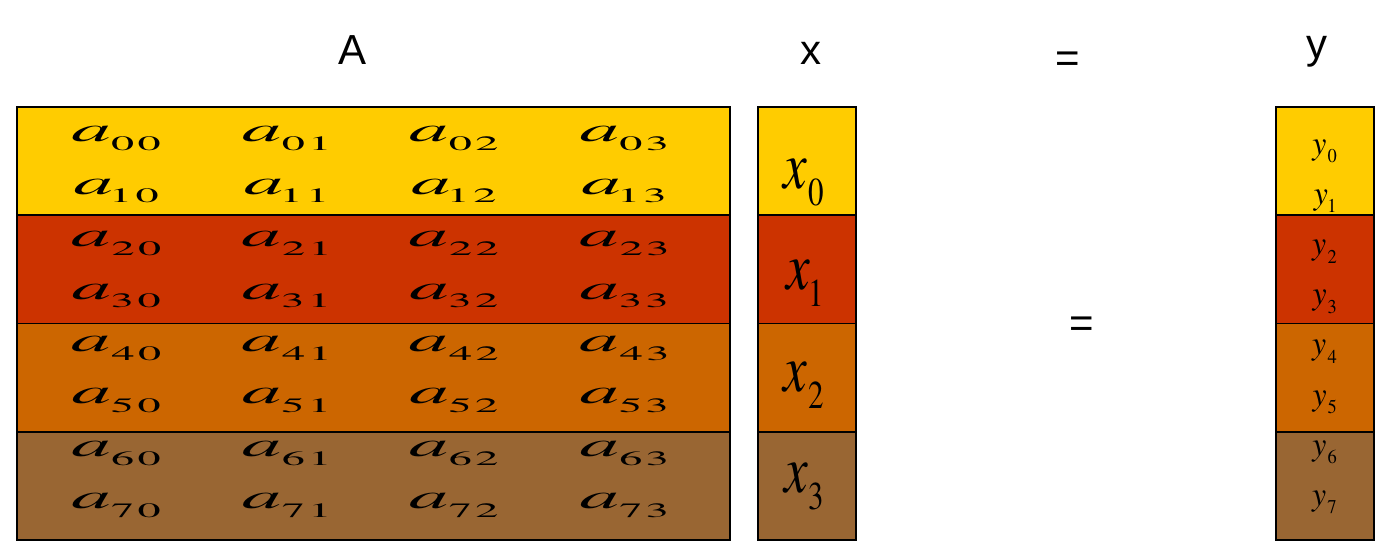
\includegraphics[width=100mm,height= 40mm]{rowbyrow.png}\hspace*{\fill}
		\caption{Row by Row distribution}
    \end{figure}
    \noindent
    The next challenge is how to construct the S matrix.  From before, S is constructed as a large tridigonal matrix, where the elements are filled in base on its positions: main diagonal, superdiagonal or subdiagonal. In this case, we are looking at chunk of the matrix S.  In other words, the dimension of each chunk is \textbf{nblocks} by \textbf{ncol}.  Each chunk can only see "ncol" column and "nblocks" row. We need a way to keep track of the coordinates of the rows. For example, if we have a 10x10 matrix and 2 processors, then the first block will have row going from 1 to 5, and then the second block will have row going from 6 to 10. The column index does not matter because it is constant across all blocks as well as the main matrix.\\

    \noindent
    To do this, the code uses two variables for the minimum and maximum row index: ILOW and IHIGH. The calculations of these ILOW and IHIGH depend on the Rank or current processor, and the number of blocks, nblocks. In the code, ILOW and IHIGH are calculed as follow:

    \begin{lstlisting}
        ILOW  = (rank*nblocks)+1
        IHIGH = (rank+1)*nblocks
    \end{lstlisting}
    \noindent
    The ILOW and IHIGH look like this in the main matrix. 


    \begin{figure}[H]
		\hfill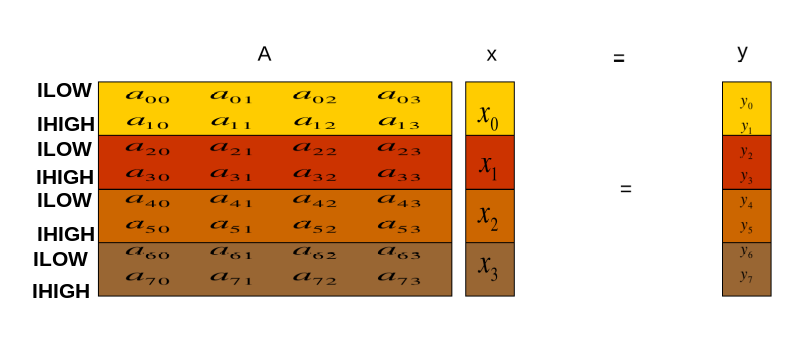
\includegraphics[width=120mm,height= 50mm]{lowhigh.png}\hspace*{\fill}
		\caption{ILOW IHIGH}
    \end{figure}



    Once these are setup, then setting up the modified tridigonal matrix is trivial. It is a matter of connecting the current row index, which ranges from ILOW to IHIGH, and the current column index, which ranges from 1 to ncol. The two special points are also added after in similar fashion. The only tricky thing here is that the first row, I = 1, only has superdiagonal element but not subdiagonal.  Consequently, the last row, I = ncol, does not have superdiagonal element. We could use ghost nodes to resolve this, or in this case, we use a couple of "if" statements to make sure that we do not access the unallocated data.  The code for this setup looks something like this:
    
    \begin{lstlisting}
    !! --------- SETTING UP S LOCAL --------------------  !!
    do i = 1, nblocks
        iTrue =i+(ILOW-1) 
        jDia = iTrue
        jSuper = jDia + 1
        jSub = jDia - 1
        
        s_local(i,:) = 0.0
        s_local(i,jDia) = 0.0

        !! PREVENT GHOST POINTS
        if (jDia /= 1) then 
            s_local(i,jSub) = 0.5
        end if 

        if (jDia /= ncol) then 
            s_local(i,jSuper) = 0.5
        end if 

        !! SPECIAL POINTS
        if (iTrue == ncol) then
            s_local(i,1) = 0.5
        end if

        if (iTrue == ncol-1) then
            s_local(i,ncol) = 1.0
        end if
    end do        
    \end{lstlisting}
    \noindent
    The X vector is setup in a similar fashion. However, this is easier because our initial guess for X is a vector with constant elements. It is important to note that creating X in this fashion will actually create a local X, not global X. Once these are setup, the matrix multiplication can then be performed, but first, we need to make sure that all processors have access to the X global. This is done by using MPIAllgather, which happens everytime we repeat the multiplication. This MPIAllgather makes sure that all processes know the entire X global in order to perform the multiplication. 

    \begin{lstlisting}
    call MPI_Allgather(x_local, nblocks,MPI_DOUBLE_PRECISION,&
        x_global,nblocks,MPI_DOUBLE_PRECISION,&
            MPI_COMM_WORLD,ierr)
    \end{lstlisting}


    \section{RESULTS}
    \subsection{SMALL PROBLEM 16 x 16 }
    \noindent
    Results are checked with different threads/proceses to make sure that the codes works.
   \hfill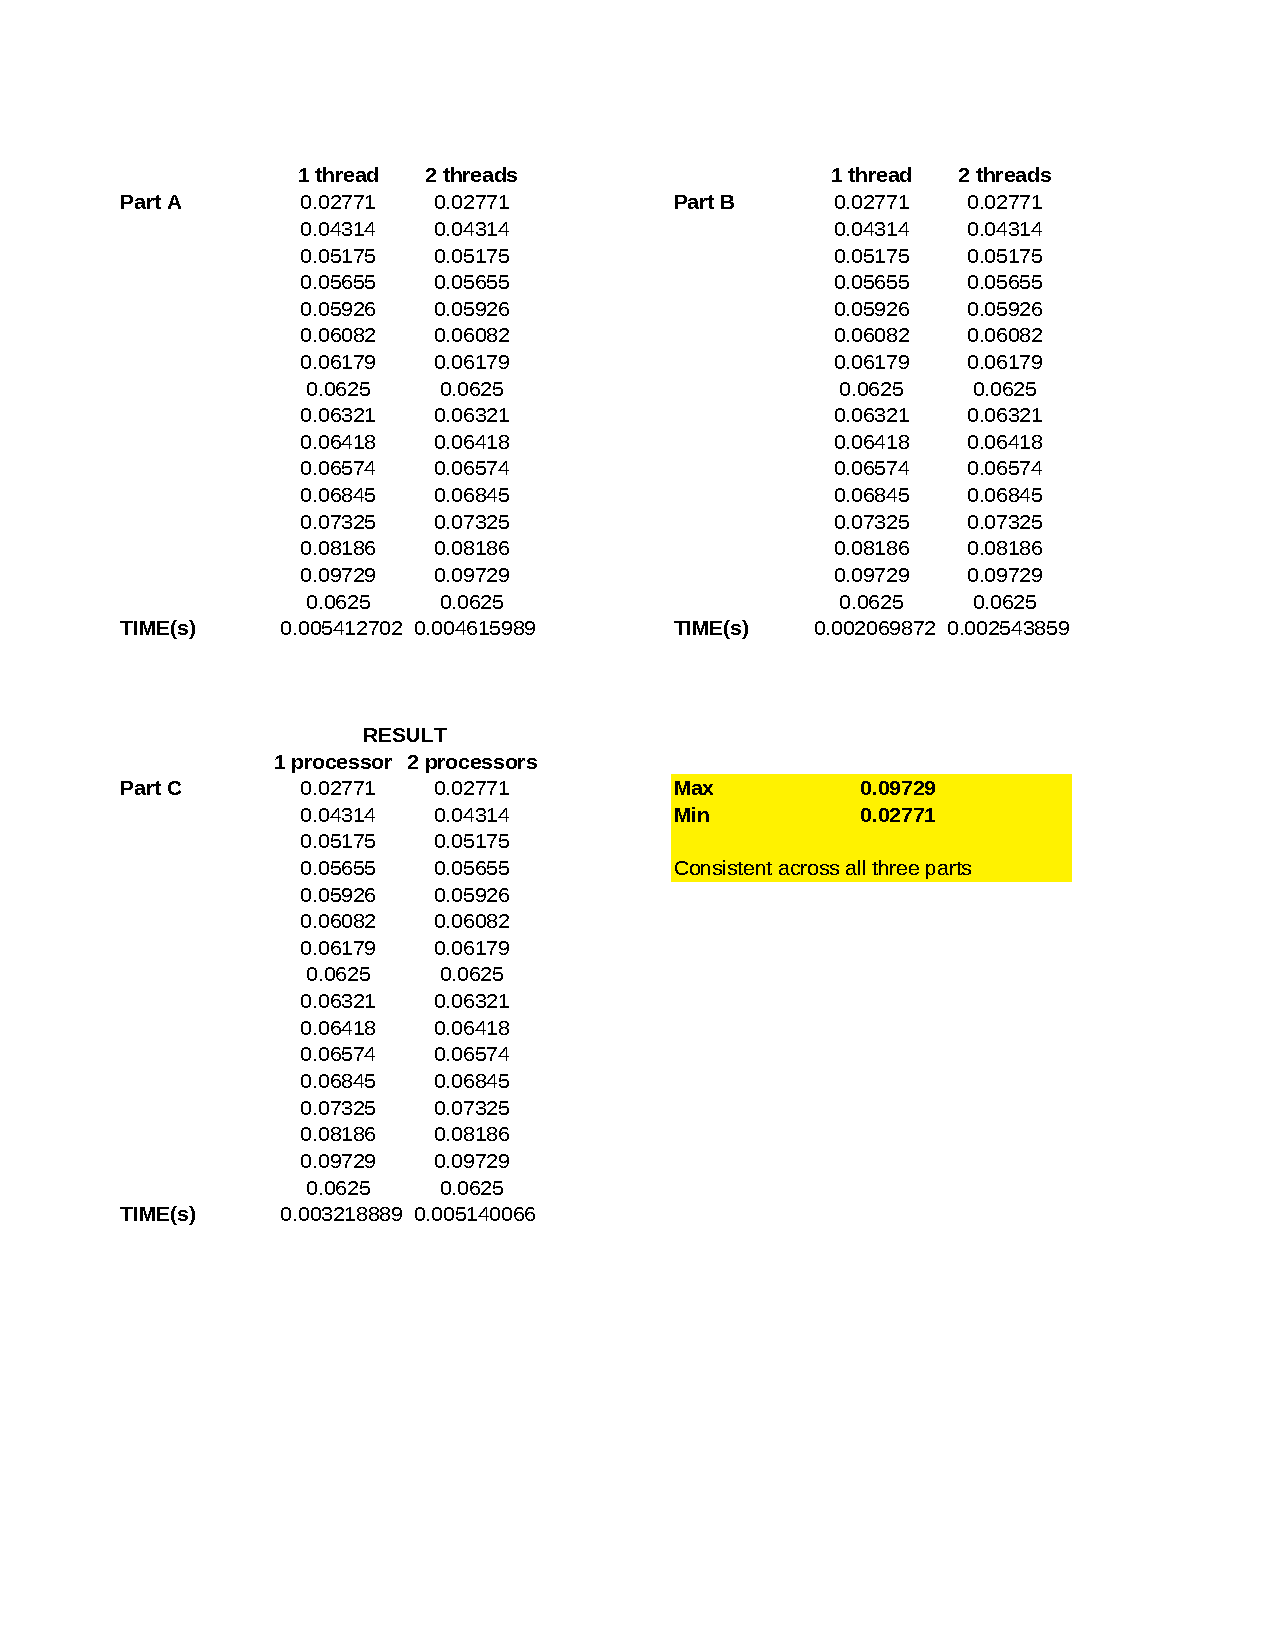
\includegraphics[width = 160mm, height = 200mm]{resultsSMALL.pdf}\hspace*{\fill}
   \newpage
   \subsection{LARGE PROBLEM 1600 x 1600}
   \noindent
   Results are recorded and speed up factors are calculated. \\
   Note: Fastest results are used for the 16 processors MPI case. 

  
   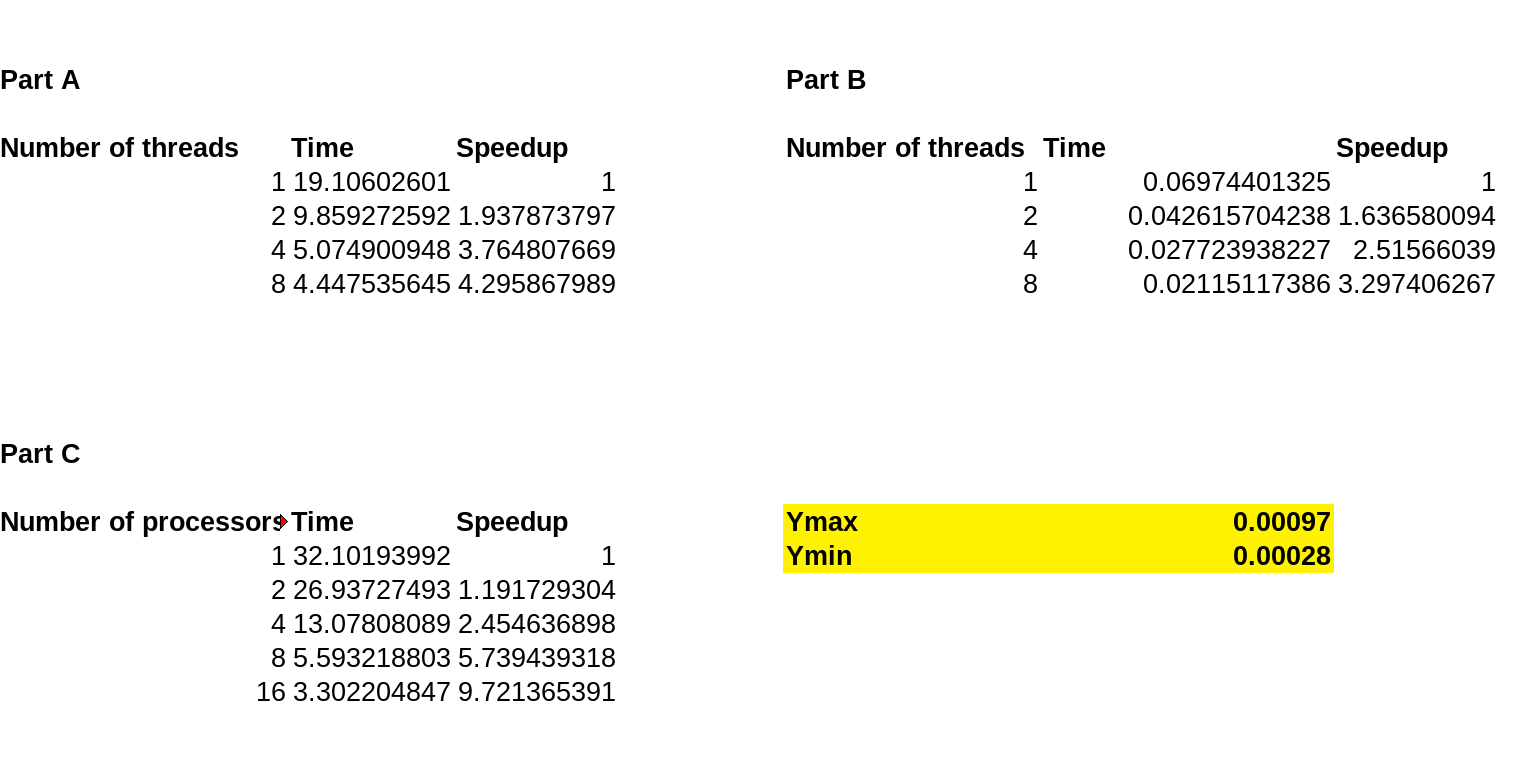
\includegraphics[height = 100mm, width = 158mm]{large.png}

   

   \noindent
   Below are the plots for the speed up factors vs number of threads/processors. 

   \begin{figure}[H]
        \hfill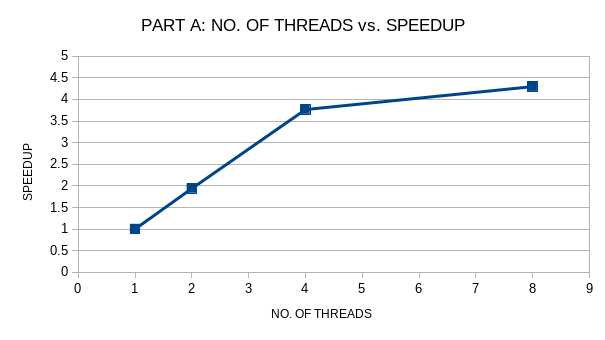
\includegraphics[width=150mm,height= 80mm]{partAplot.png}\hspace*{\fill}
        \caption{No. of threads vs Speedup for part A}
    \end{figure}


    \begin{figure}[H]
        \hfill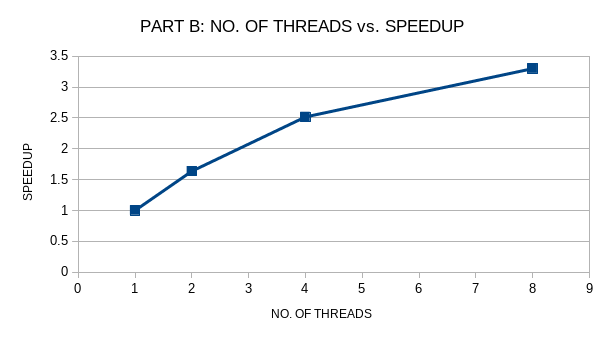
\includegraphics[width=150mm,height= 80mm]{partBplot.png}\hspace*{\fill}
        \caption{No. of threads vs Speedup for part B}
    \end{figure}


    \begin{figure}[H]
        \hfill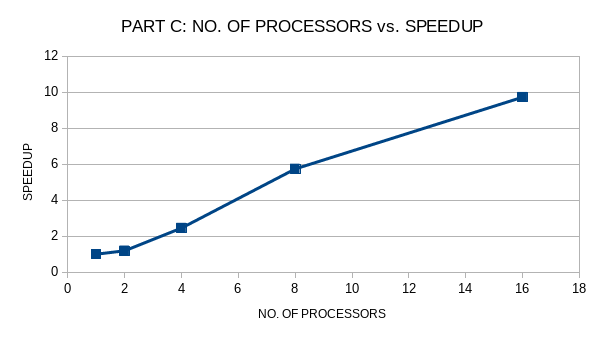
\includegraphics[width=150mm,height= 80mm]{partCplot.png}\hspace*{\fill}
        \caption{No. of processors vs Speedup for part C}
    \end{figure}

    \iffalse
    \newpage
    \noindent
    It is interesting to note that the Intel version of the MPI FORTRAN gives better results. 

    \hfill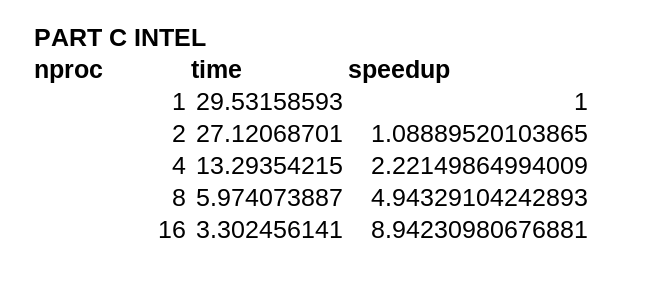
\includegraphics[height = 40mm, width = 90mm]{intel.png}\hspace*{\fill}

    \noindent
    Of course, comparing the two speedup factors shows that the Intel FORTRAN MPI is way better. The GNU MPI Compiler gives faster execution time with each added thread; however, there are no visible improvements compare to the 


    \begin{figure}[H]
        \hfill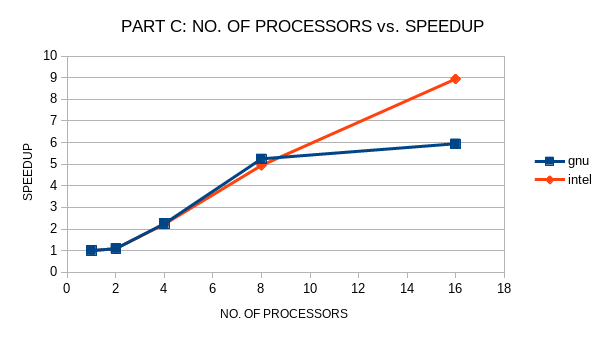
\includegraphics[width=150mm,height= 80mm]{partC_COMBINE.png}\hspace*{\fill}
        \caption{No. of processors vs Speedup for part C}
    \end{figure}
    \fi

   \newpage
   \section{DISCUSSIONS}
   \subsection{SPEED UP COMPARISON}
   Generally, perfect speed up occurs when speedup factor = Number of threads/processors.  For the dense OPENMP version, perfect speed up is almost reached when running at 2 threads. As we increase the number of threads, we see speed up but these are not significant enough for "perfect speedups". It looks like using 4 threads is the bottleneck for the BlueShark cluster. This is because after 4 threads, we do not see any further improvement in terms of speed up. On the other hand, the sparse CSR OPENMP version is significantly faster than the dense OPENMP version.  This is easy to understand because CSR only stores the non zero elements. In our problems, we have very few of these non zero elements. Thus, the code only has to perform very few multiplications. Unfortunately, the speed up factor is not that great compare to the dense OPENMP version.  Perhaps, a larger problem size will tell us more about the advantage of CSR. A possible explanation for this would be that the CSR version only deals with non zero elements. In our setup, the tridigonal matrix has very few of these "non zero elements".  Therefore, the BlueShark cluster has no problem running the code on 1 thread. We can see clearly that the time to run 1 thread for the CSR code is almost 100 times faster than the dense OPENMP. For 1 thread, there are no problems for CSR; therefore, more threads will be faster but it is not significant enough for us to capture the speedups. Lastly, the MPI version, although not as fast as the CSR code, shows considerable speedup up to 8 processors. With 16 processors, we seem to reach a limit and the reason for this might be that BlueShark only has 12 processors; if we ask for more than 12 then there will be problems in communications. Even so, "perfect speedup" is almost achieved when we have 2 processors. Again, larger problem size will help us to see and have better judgements on the speedups. Additionally, we can also look into the case when the number of pages is not a multiple of number of processors for the MPI version. In that case, we have to look at what to do with the remainders. However, our speedups in that case will not be as high. \\
   It is also important to note that with 16 processors for the MPI version, the results are mixed. The reason for this could be that BlueShark is trying to access more than 12 cores. The fastest result is used for the 16 processor case.  
   \subsection{APPROACH COMPARISON}
   In terms of programming effort, the dense OPENMP is the easiest to code while the MPI version is the hardest to implement. In terms of performance, CSR approach gives the fastest executions, while the MPI vesion gives the similar execution time as the dense OPENMP. However, in my opinion,this is not a fair comparision. The reason is that MPI version gets to use around 16 processors; while the OPENMP can only use up to 8 threads. A better improvemen to the assignment is to run these codes on a cluster where there are no limits on the number of cores (12 cores for BlueShark). CSR is tricky when we have to implement the A, jA, and iA arrays.  Our timing does not include this portion of the code; I believe that this is significant because we have to form the S matrix then break it down to three special arrays.  It takes a lot of resources to check if there are non zero elements and then store those.  From the way we time our code, it could be said that we assumed that these special arrays are given, we just need to perform the multiplications.  It is trivial that these CSR multiplications will be much faster because we only multiply a few non zero elements. 

   \newpage
   \section{CODES (all .f95 compile via gfortran and mpif90)}
   \subsection{PART A CODES}


   \begin{lstlisting}
    program partA
    use omp_lib
    implicit none

    ! PROBLEM VARIABLES
    real*8,dimension(:,:),allocatable :: s2d,bmat,gmat
    real*8,dimension(:),ALLOCATABLE :: gmat1d,x_vector,y_vector
    integer :: ncol = 1600
    integer :: nshape 
    integer :: i,j
    real*8 :: q
    integer :: timecount
    DOUBLE PRECISION :: tstart,tend,timeelapse
    CHARACTER :: np
    REAL*8 :: sumi

    !OPEN MP VARIABLES

    integer :: num_threads


    !----------------  SETTING UP S-----------------------------!
    interface 
        subroutine formS(nsize,smat)
            implicit none
            integer,INTENT(IN) :: nsize
            real*8,INTENT(OUT),DIMENSION(:,:),ALLOCATABLE :: smat

        end subroutine formS
    end interface

    num_threads = 4
    call omp_set_num_threads(num_threads)


    !CALL get_environment_variable("OMP_NUM_THREADS", np)
    !num_threads = ICHAR(np)
    !read(np, *) num_threads
    !call omp_set_num_threads(num_threads)
    
    !num_threads = omp_get_num_threads()    

    !print*, "Running with ", num_threads, " threads ", np


    allocate(s2d(ncol,ncol))
    call formS(ncol,s2d)    

    !----------------  END SETTING UP S------------------------!




    !----------------  SETTING UP G----------------------------!

    q = 0.15

    allocate(bmat(ncol,ncol))

    ! First, setup Bmatrix, each element = 1/numPage
    bmat(:,:) = 1.00/ncol



    ! Now, forming G
    allocate(gmat(ncol,ncol))
    !gmat = (1.00-q)*s2d + q*bmat 


    do i = 1,ncol
        do j = 1,ncol
            gmat(i,j) = (1.00-q)*s2d(i,j) + q*bmat(i,j)
        end do
    end do
    

    ! Convert G into 1d
    nshape = ncol**2
    allocate(gmat1d(nshape))
    gmat = transpose(gmat)
    gmat1d = reshape(gmat, [nshape] ) 

    !----------------  END SETTING UP G------------------------!



    !----------------  SETTING UP X----------------------------!


    allocate(x_vector(ncol))
    x_vector(:) = 1.00/ncol

    allocate(y_vector(ncol))  !set up y_vector as well
    y_vector(:) = 0.0   ! zero out   

    !----------------  END SETTING UP X------------------------!




    !----------------- MAIN MATVEC ----------------------------!

    tstart =  omp_get_wtime()
    
    do timecount = 1,1000
	!$OMP PARALLEL DO private(sumi)
        do i = 1,ncol
 	    sumi = 0.0
            do j = 1,ncol
                sumi = sumi + gmat1d((i-1)*ncol+j)*x_vector(j)
            end do
	    y_vector(i) = sumi
        end do  
	!$OMP END PARALLEL DO
        
        !$OMP DO
        do i = 1,ncol
            x_vector(i) = y_vector(i)  !UPDATE X
        end do
        !$OMP END DO
    end do
   
    tend =  omp_get_wtime()
    
    timeelapse = tend-tstart

    
    !----------------- END MAIN MATVEC ---------------------!


    
    if (ncol == 16) then 

        write(6,*) "-----------------------------------------"


        WRITE(6,*) " Y = "
        do i = 1,ncol
            write(6,20) y_vector(i)
            20 format('  ',F7.5)
        end do

        write(6,*) " "

        write(6,*) "YMAX = "
        WRITE(6,25) MAXVAL(y_vector)
        25 format('  ',F7.5)


        write(6,*) " "

        write(6,*) "YMIN =  "
        WRITE(6,26) MINVAL(y_vector)
        26 format('  ',F7.5)



        write(6,*) " "

        write(6,*) " Time Elapsed ="
        write(6,30) timeelapse
        30 format(F16.12)

        write(6,*) "-----------------------------------------"
    else
        write(6,*) "-----------------------------------------"

        write(6,*) "YMAX = "
        WRITE(6,31) MAXVAL(y_vector)
        31 format('  ',F7.5)


        write(6,*) " "

        write(6,*) "YMIN =  "
        WRITE(6,32) MINVAL(y_vector)
        32 format('  ',F7.5)

        write(6,*) " "

        write(6,*) " Time Elapsed ="
        write(6,33) timeelapse
        33 format(F16.12)

        write(6,*) "----------------------------------------"
    end if

    !----------------- END MAIN MATVEC ---------------------!



    !! DEALLOCATE 
    deallocate(gmat)
    deallocate(bmat)
    deallocate(s2d)
    
end program partA 



subroutine formS(nsize,smat)
    implicit none
    integer ::  icol
    integer,INTENT(IN) :: nsize
    
    real*8,INTENT(OUT),DIMENSION(:,:),ALLOCATABLE :: smat


    ALLOCATE(smat(nsize,nsize))

    !Super diagonal
    do icol = 1,nsize-1 !loop row
       
        smat(icol,icol+1) = 0.5
      
    end do

    !Sub diagonal

    do icol = 2,nsize
        smat(icol,icol-1) = 0.5
    end do
   
    smat(nsize,1) = 0.5
    smat(nsize-1,nsize) = 1

end subroutine







   \end{lstlisting}



   \newpage
   \subsection{PART B}

   \begin{lstlisting}
    program partB
    use omp_lib
    implicit none

    ! PROBLEM VARIABLES
    real*8,dimension(:,:),allocatable :: s2d
    real*8,dimension(:),ALLOCATABLE :: x_vector,y_vector
    integer :: ncol = 1600
    real*8 :: q= 0.15
    integer :: timecount
    integer :: nshape
    DOUBLE PRECISION :: tstart, tend, timetaken 
    real*8 :: Sxsumi


    ! CSR STUFF

    REAL*8,DIMENSION(:),ALLOCATABLE :: a_vec
    INTEGER,DIMENSION(:),ALLOCATABLE :: j_vec
    INTEGER,DIMENSION(:),ALLOCATABLE:: i_vec
    INTEGER,DIMENSION(:),ALLOCATABLE :: nsizezero
    INTEGER :: nsize, counter
    INTEGER :: i,j,k


    ! OMP VARIABLES
    integer :: num_threads
    character :: np


    !----------------  SETTING UP S------------------------!
    interface 
        subroutine formS(nsize,smat)
        implicit none
        integer,INTENT(IN) :: nsize
        real*8,INTENT(OUT),DIMENSION(:,:),ALLOCATABLE :: smat
        end subroutine formS
    end interface  

   
   num_threads = 1
   call omp_set_num_threads(num_threads)

    
    allocate(s2d(ncol,ncol))
    call formS(ncol,s2d)  


    !----------------  FORMING CSR ----------------------!

    nsize = count (s2d/=0)      ! FIND # of NON ZEROS in S
    ALLOCATE(nsizezero(ncol))
    ALLOCATE(a_vec(nsize))      ! A has length # of non zero
    ALLOCATE(j_vec(nsize))      ! J has length # of non zero
    ALLOCATE(i_vec(ncol+1))     ! I has length NCOL+1

    counter = 1


    ! CALCULATE A, and jA, get non zero in each row
    do i = 1,ncol
        nsizezero(i) = count(s2d(i,:)/=0)
        do j = 1,ncol
            if (s2d(i,j) /= 0) then 
                a_vec(counter) = s2d(i,j)
                j_vec(counter) = j
                counter = counter + 1
            end if
        end do
    end do

    i_vec(1) = 1
    do i = 2,ncol+1
        i_vec(i) = i_vec(i-1) + nsizezero(i-1)
    end do



    !----------------  SETTING UP X----------------------!


    allocate(x_vector(ncol))
    x_vector(:) = 1.00/ncol

    allocate(y_vector(ncol))  !set up y_vector as well
    y_vector(:) = 0.0   ! zero out   

  

    !-----------------  MAIN MULTIPLY ------------------!

    ! ALLOCATE(Sx_vector(ncol))       ! to store (1-q)Sx
    tstart =  omp_get_wtime()
    do timecount = 1,1000
        !$OMP PARALLEL DO private(Sxsumi)
        do i = 1,ncol
            Sxsumi = 0.0
            
            do k = i_vec(i),i_vec(i+1)-1
                Sxsumi = Sxsumi+a_vec(k)*x_vector(j_vec(k))
            end do
            
            y_vector(i) = (1-q)*Sxsumi + q/ncol
        end do
        !SOMP END PARALLEL DO

        !$OMP DO 
        ! Update X 
        do i = 1,ncol
            x_vector(i) = y_vector(i)
        end do
        !$OMP END DO
        
    end do

    tend =  omp_get_wtime()

    timetaken = tend-tstart


    if (ncol == 16) then 

        write(6,*) "---------------------------------------"


        WRITE(6,*) " Y = "
        do i = 1,ncol
            write(6,20) y_vector(i)
            20 format('  ',F7.5)
        end do

        write(6,*) " "

        write(6,*) "YMAX = "
        WRITE(6,25) MAXVAL(y_vector)
        25 format('  ',F7.5)


        write(6,*) " "

        write(6,*) "YMIN =  "
        WRITE(6,26) MINVAL(y_vector)
        26 format('  ',F7.5)



        write(6,*) " "

        write(6,*) " Time Elapsed ="
        write(6,30) timetaken
        30 format(F16.12)

        write(6,*) "-------------------------------------"

    else
        write(6,*) "-----------------------------------"

        write(6,*) "YMAX = "
        WRITE(6,31) MAXVAL(y_vector)
        31 format('  ',F7.5)


        write(6,*) " "

        write(6,*) "YMIN =  "
        WRITE(6,32) MINVAL(y_vector)
        32 format('  ',F7.5)

        write(6,*) " "

        write(6,*) " Time Elapsed ="
        write(6,33) timetaken
        33 format(F16.12)

        write(6,*) "--------------------------------------------"
    end if

            

    !! DEALLOCATE ARRAYS
    DEALLOCATE(y_vector)
    DEALLOCATE(x_vector)
    DEALLOCATE(j_vec)
    DEALLOCATE(a_vec)
    DEALLOCATE(i_vec)
    DEALLOCATE(s2d)
    DEALLOCATE(nsizezero)


end program partB



subroutine formS(nsize,smat)
    implicit none
    integer ::  icol
    integer,INTENT(IN) :: nsize
    
    real*8,INTENT(OUT),DIMENSION(:,:),ALLOCATABLE :: smat


    ALLOCATE(smat(nsize,nsize))

    !Super diagonal
    do icol = 1,nsize-1 !loop row
       
        smat(icol,icol+1) = 0.5
      
    end do

    !Sub diagonal

    do icol = 2,nsize
        smat(icol,icol-1) = 0.5
    end do
   
    smat(nsize,1) = 0.5
    smat(nsize-1,nsize) = 1

end subroutine

       
   \end{lstlisting}

   \newpage
   \subsection{PART C}

   \begin{lstlisting}
    program partC
    ! use mpi
     include 'mpif.h'
    ! implicit none
 
     !! DECLARE PROBLEM VARIABLES
 
     integer :: i,j,iTrue,k
     DOUBLE PRECISION,dimension(:,:),ALLOCATABLE:: s_local, &
        s_global, b_local, b_global, g_local, g_global
     DOUBLE PRECISION :: q = 0.15
     DOUBLE PRECISION,DIMENSION(:), ALLOCATABLE :: x_local, &
        y_local, y_global, x_global
     integer :: ncol = 1600
  
     integer :: timecount 
 
     DOUBLE PRECISION :: ymin, yminlocal
 
     DOUBLE PRECISION :: ymax, ymaxlocal
 
     DOUBLE PRECISION :: tstart,tend,timeelapse
  
     !! DECLARE MPI VARIABLES
     integer :: rank,nprocs,ierr
 
 
 
     !! DECLARE OTHER VARIABLES
     integer :: IHIGH,ILOW
     integer :: nblocks
     integer :: jDia, jSuper, jSub
 
 
 
     !Start MPI
     call MPI_INIT(ierr)
     call MPI_COMM_SIZE(MPI_COMM_WORLD,nprocs,ierr)
     call MPI_COMM_RANK(MPI_COMM_WORLD,rank,ierr)
 
 
 
 
 
     nblocks = FLOOR(REAL(ncol/nprocs))
 
     ALLOCATE(s_local(nblocks,ncol))
     ALLOCATE(b_local(nblocks,ncol))
     ALLOCATE(g_local(nblocks,ncol))
     ALLOCATE(x_local(nblocks))
     ALLOCATE(y_local(nblocks))
     ALLOCATE(y_global(ncol))
     ALLOCATE(x_global(ncol))
 
 
     ! ROW COORDINATES FOR EACH SUB BLOCK
     ILOW  = (rank*nblocks)+1
     IHIGH = (rank+1)*nblocks
 
     do i = 1, nblocks
 
         ! --------- SETTING UP S LOCAL ----------!
         iTrue =i+(ILOW-1) 
         jDia = iTrue
         jSuper = jDia + 1
         jSub = jDia - 1
         
         s_local(i,:) = 0.0
         s_local(i,jDia) = 0.0
     
         !! Special cases
         if (jDia /= 1) then 
             s_local(i,jSub) = 0.5
         end if 
 
         if (jDia /= ncol) then 
             s_local(i,jSuper) = 0.5
         end if 
 
 
         if (iTrue == ncol) then
             !! More special points
             s_local(i,1) = 0.5
         end if
 
 
         if (iTrue == ncol-1) then
             !! More special points 
             s_local(i,ncol) = 1.0
         end if
 
 
         !----------- SETTING UP Y LOCAL ---------!
         y_local(:) = 0.0
     end do
 
     do i=1,nblocks
 
        !------------ SETTING UP X LOCAL----------!
 
         x_local(i) = 1.00/ncol
     end do
 
 
 
 
 
     tstart = MPI_WTIME()    
     do timecount = 1,1000
 
         call MPI_Allgather(x_local, nblocks,&
         MPI_DOUBLE_PRECISION,x_global,nblocks,&
            MPI_DOUBLE_PRECISION,MPI_COMM_WORLD,ierr)
 
 
         do i = 1,nblocks
             y_local(i) = 0.0
 
             do j = 1,ncol
                 y_local(i) = y_local(i) + (1-q)*s_local(i,j)&
                    *x_global(j)                 
             end do
             y_local(i) = y_local(i) + (q/DBLE(ncol)) 
 
         end do
 
         !   UPDATE X 
         do k = 1,nblocks
             x_local(k) = y_local(k)
         end do
     end do
     tend = MPI_WTIME()         
 
 
 
     !!------------ CALCULATE MAX  and MIN
     ymaxlocal = maxval(y_local) 
     call MPI_Reduce(ymaxlocal,ymax,1,MPI_DOUBLE_PRECISION,&
        MPI_MAX, 0, MPI_COMM_WORLD,ierr)
 
 
     
     yminlocal = minval(y_local) 
     call MPI_Reduce(yminlocal,ymin,1,MPI_DOUBLE_PRECISION,&
        MPI_MIN, 0, MPI_COMM_WORLD,ierr)
 
    
 
     if (ncol == 16) then 
     call MPI_Allgather(y_local, nblocks,MPI_DOUBLE_PRECISION,&
     y_global,nblocks,MPI_DOUBLE_PRECISION,MPI_COMM_WORLD,ierr)
         if (rank == 0 ) then 
             
             WRITE(6,*) " Y = "
             do i = 1,ncol
                 write(6,20) y_global(i)
                 20 format('  ',F7.5)
             end do
 
             write(6,*) "YMAX = "
             WRITE(6,25) ymax
             25 format('  ',F7.5)
 
 
             write(6,*) " " 
 
             write(6,*) "YMIN =  "
             WRITE(6,26) ymin
             26 format('  ',F7.5)
 
             write(6,*) " Time Elapsed ="
             write(6,30) (tend-tstart)
             30 format(F16.12)
 
 
 
                 
 
         end if
      
    else 
 
         if (rank == 0 ) then 
 
             write(6,*) "YMAX = "
             WRITE(6,31) ymax
             31 format('  ',F7.5)
 
 
             write(6,*) " " 
 
             write(6,*) "YMIN =  "
             WRITE(6,32) ymin
             32 format('  ',F7.5)
             
             
             write(6,*) " Time Elapsed ="
             write(6,33) (tend-tstart)
             33 format(F16.12)
 
 
         end if
     end if 
     
 
 
     DEALLOCATE(s_local)
     DEALLOCATE(b_local)
     DEALLOCATE(g_local)
 
 
     !Stop MPI
     call MPI_FINALIZE(ierr)
 
 
 
 
 
 
 end program partC
 
       
   \end{lstlisting}







    


    
    



    

\end{document}